The \texttt{\pkglnk{model.output}} package contains the \texttt{\lnk{OutputSize}} interface, all
its implementations that the model provides and the \texttt{\lnk{OutputSizes}} static
class.

\texttt{\lnk{OutputSize}} is implemented by policies that decide which lambda terms should be
displayed to the user based on their step numbers. For deciding which terms should
be displayed after execution has finished, the total number of steps and the number of
the last term that was displayed while the execution was still running is taken into
account.

The policies provided by the model show every term (\texttt{\lnk{Full}}), only every
$n$-th term for some $n$ (\texttt{\lnk{Periodic}}), only the first $n$ and last $n$ terms
for some $n$ (\texttt{\lnk{Shortened}}) or only the very last term (\texttt{\lnk{ResultOnly}}).

Similarly to the analogous classes in the \texttt{\pkglnk{model.reduction}} and \texttt{\pkglnk{model.library}} packages,
\texttt{\lnk{OutputSizes}} provides instances of the aforementioned classes.

\begin{figure}[H]
	\centering
	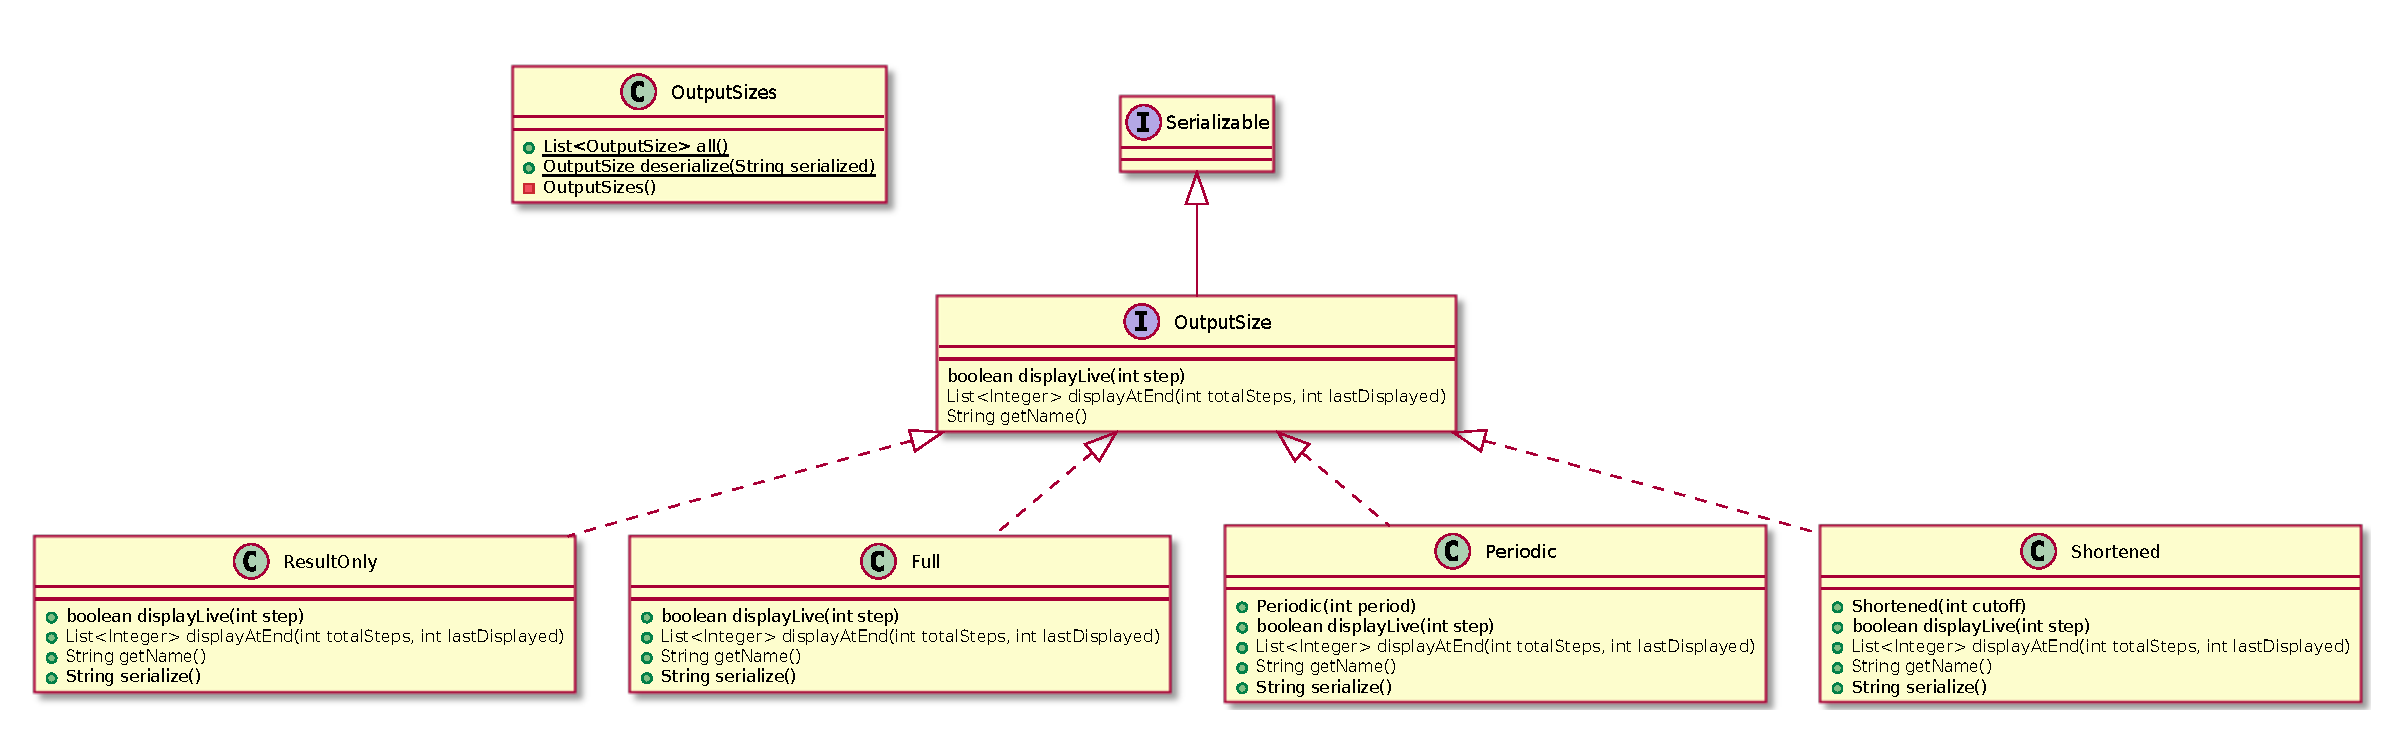
\includegraphics[width=\textwidth]{packageDiagrams/modelOutputPackage}
\end{figure}
